\documentclass{IEEEtran}
%% BIbliography Setup - Biblatex please
\usepackage[
backend=biber,
style=ieee,
]{biblatex}
\addbibresource{DBT_References.bib}

%% Packages
\usepackage{caption}
\usepackage [none] {hyphenat} 
\usepackage{siunitx}
\usepackage{graphicx}
\usepackage{amsmath}
\usepackage{subcaption}
\usepackage{pdfpages}
\usepackage{booktabs}
\usepackage{svg}

\markboth{First National Conference On Advanced Materials and their Applications , October 18 and 19 th 2023 Tipaza}{Last Name \MakeLowercase{\textit{et al.}}: Title}

\title{CDT 22 - Design, Build and Test. Sequential Instabilities for Actuating Aerodynamic Surfaces}
\author{First Author$^1$, Second Author$^2$, and Third Author$^3$\\
	$^1$Department of Electrical Engineering, University of X, X City, X Country\\
	$^2$Department of Computer Science, University of Y, Y City, Y Country\\
	$^3$Department of Mechanical Engineering, University of Z, Z City, Z Country\\
	\{first.author, second.author, third.author\}@cu-tipaza.dz}
\begin{document}
	\maketitle
	
	\begin{abstract}
		
	\end{abstract}
	
	\section{Introduction}
		\subsection{Control Surfaces for Gust Load Alleviation}
		Gust loads are well known as a source of potential catastrophic failure in aircraft structures; with rare, extreme gusts in particular being a source of the maximum loads that an aircraft may experience. \cite{Wu2019,Guo_2015}. Aircraft structural requirements are driven by extreme cases to prevent failure, despite operating in far less intense loading environments for the majority of the aircraft's service life \cite{Li2021}. The added capability to cope with extreme gust loads is unnecessary most of the time and comes with an associated parasitic mass increase, which causes reduced fuel efficiency of the aircraft. 
		
		Gust load alleviation (GLA) systems aim to reduce the effect of gust loads while minimising mass increase by altering the aerodynamic profile of the wing \cite{Li_2022}. Active control surfaces such as ailerons, spoilers have been used to achieve this \cite{Li_2022}. However, such control surfaces utilise conventional, active actuation mechanisms such as hydraulic or electro-mechanical actuators \cite{QI_2011}. These mechanisms still introduce significant mass and complexity to aircraft which still results in a decrease to fuel efficiency and an increase in cost and manufacture time. A passively actuated GLA system is a mechanism which is able to deploy using the deformation of the wing itself. These are attractive as they are typically simpler and require no external energy \cite{Li_2022}. A lightweight, passive GLA system could provide the necessary gust alleviation whilst keeping the parasitic mass added to the aircraft low.  
		
		\subsection{Sequential Instabilities}
		A potential actuation mechanism for a passive GLA system is through the utilisation of structural instabilities. The traditional view on structural instability, known as '\textit{Buckliphobia}', is largely negative and the presence of buckling is seen as a failure mode. '\textit{Buckliphillia}' is an emerging design philosophy which seeks to exploit instability as a design feature \cite{Reis_2015}. By deliberately designing a structure to become unstable in predictable ways, useful functionality can be achieved, such as large and rapid deflections in shape morphing structures. This approach has potential application for aircraft design as the deflections necessary for actuating a control surface could be achieved through a '\textit{Buckliphillic}' approach. Examples of structural instability exploited for functionality in control surface actuation include: A bistable composite trailing edge flap \cite{Daynes2010} and a non-linear spring wing-tip device for gust load alleviation \cite{Castrichini2017}.
		
         By extending this approach to include the exploitation of interacting instabilities, new interesting and novel designs for dynamic structures can be produced. Buckling modes are able to interact with each other and interacting instabilities occur when two or more buckling modes share coincident critical points \cite{Wheatcroft_2023}. Whilst the adoption of structural instability as a design feature has received much attention in recent years and shifted the view of instability to be more positive, interacting instabilities are still viewed primarily as a failure mechanism. A novel concept for a passively-actuated spoiler proposed by Wheatcroft et al. exploits sequential, interacting instabilities to produce a large post buckling deflection in a bistable, constant curvature, composite laminate \cite{Wheatcroft_2023}. A pair of instabilities can be considered sequential when an instability in one system triggers a subsequent instability in another. Utilising sequential instability as a design feature enables refined control over the device deployment, whilst eliminating the need for heavy, active deployment mechanisms.
		
		\subsection{Pop-up Spoiler Concept}
		\begin{figure}[!h]
			\centering
			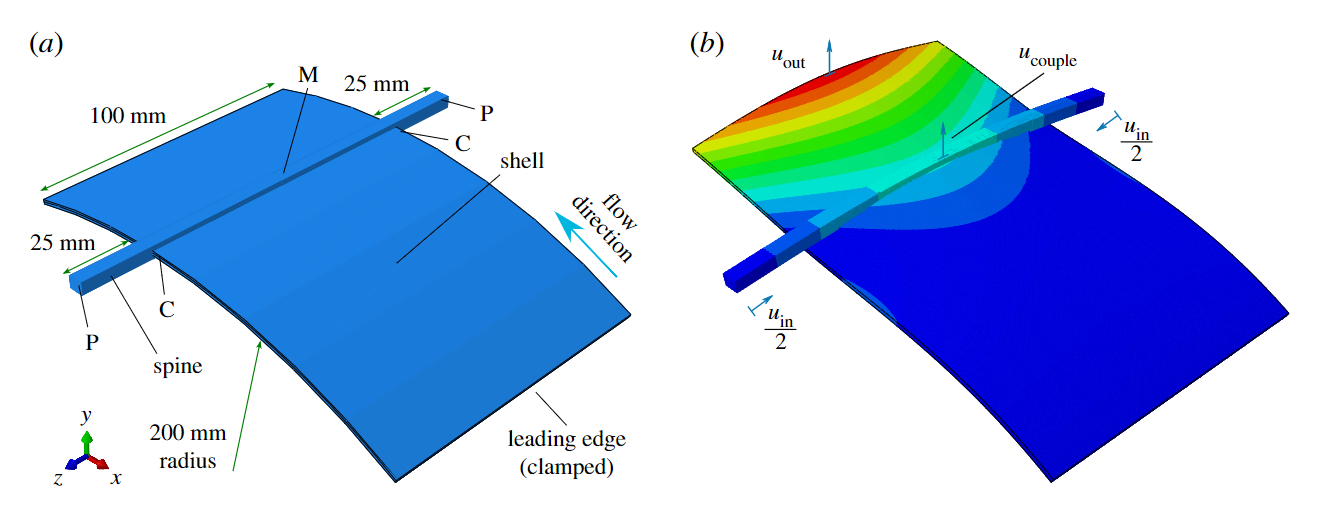
\includegraphics[width=0.45\textwidth]{IntroductionImages/Concept.png}
			\caption{FE model of original concept for passively actuated pop-up spoiler, \textbf{(a)}: undeployed state, \textbf{(b)} deployed state. (Taken from \cite{Wheatcroft_2023})}
			\label{fig:OGConcept}
		\end{figure}
	
		The original novel spoiler concept proposed by Wheatcroft et al. is shown in Figure \ref{fig:OGConcept} and is constituted from an Euler strut and a bistable composite laminate. In the original work the laminate is a constant curvature. For this investigation, the concept is extended to include a composite laminate shaped to the upper surface of an aerofoil to better resemble the application for a wing mounted spoiler. It is envisioned that strain caused by deflection in a wing under heavy load will cause the strut to buckle into a mode that subsequently causes the laminate to buckle, creating a sequential instability. A representative bar and spring diagram for this system is shown in Figure \ref{fig:BarNSpring}. From this diagram the deployment mechanism which exploits the  interaction between the a pair of instabilities can clearly be seen. This should produce the ideal behaviour, shown in Figure XX, where the deflection of the laminate, $u_out$, is plotted as a function of the enforced axial compressive deformation of the Euler strut, $u_in$. Once $u_in$  reaches a critical value it results in the system traversing an unstable region, resulting in a dynamic deflection.

		\begin{figure}[!h]
			\centering
			\includesvg[width=0.45\textwidth]{IntroductionImages/vK-Strut_V2.svg}
			\caption{Bar and spring model representing the sequential instability system of the concept. (Reprinted from \cite{Wheatcroft_2023})}
			\label{fig:BarNSpring}
		\end{figure}
	
		\begin{figure}[!h]
			\centering
			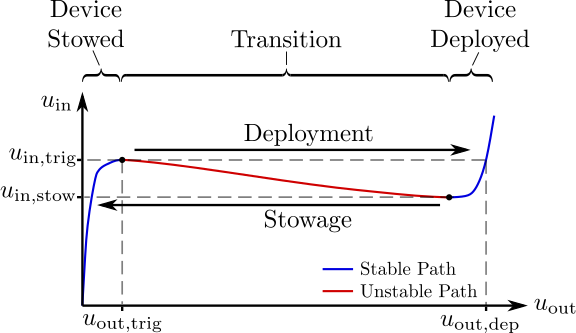
\includegraphics[width=0.45\textwidth]{IntroductionImages/Desired_Path_V4.png}
			\caption{Ideal behaviour of the passively actuated spoiler concept. (Reprinted from \cite{Wheatcroft_2023})}
			\label{fig:DesiredPath}
		\end{figure}
	
		
	\section{Methodology}
		
	\subsection{Equations}
	Here is an example of an equation:
	\begin{equation}
		f(x) = x^2 + 2x + 1
	\end{equation}
	
	\subsection{Tables}
	Here is an example of a table:
	\begin{table}[htbp]
		\centering
		\caption{Example Table}
		\label{tab:example}
		\begin{tabular}{|c|c|c|}
			\hline
			\textbf{Column 1} & \textbf{Column 2} & \textbf{Column 3} \\
			\hline
			Row 1, Column 1 & Row 1, Column 2 & Row 1, Column 3 \\
			\hline
			Row 2, Column 1 & Row 2, Column 2 & Row 2, Column 3 \\
			\hline
			Row 3, Column 1 & Row 3, Column 2 & Row 3, Column 3 \\
			\hline
		\end{tabular}
	\end{table}
	
	\subsection{Figures}
	Here is an example of a figure:
	\begin{figure}[htbp]
		\centering
		\includegraphics[width=0.4\textwidth]{example-image-a}
		\caption{Example Figure}
		\label{fig:example}
	\end{figure}
	
	\section{Results}
	
	\section{Conclusion}
	
	
    \printbibliography
	
\end{document}

%%TEMPLATES
%%PNG or JPEG files
\begin{figure}[!h]
	\centering
	\includegraphics[height=8cm]{}
	\caption{Caption}
	\label{fig:}
\end{figure}
%% SVG Files
\begin{figure}[!h]
	\centering
	\includesvg[height=8cm].svg}
	\caption{Caption}
	\label{fig:}
\end{figure}